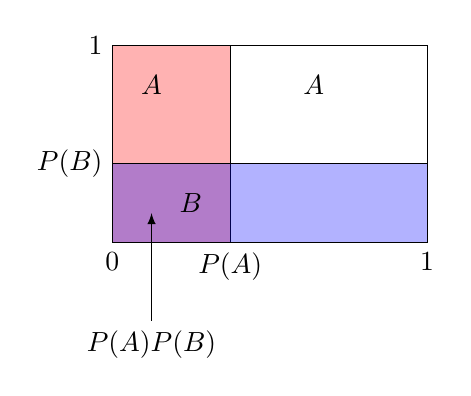
\begin{tikzpicture}[scale=0.5]

\draw  (-4,3)  rectangle (-4,3);
\draw  (-8,6) coordinate (v1) rectangle (0,1) node (v2) {};
\begin{scope}[fill opacity=0.3]
\draw[fill=red]  (v1) rectangle (-5,1);
\draw[fill=blue]  (-8,1) rectangle (0,3);
\end{scope}



\node at (-7,5) {$A$};
\node at (-3,5) {$~A$};
\node at (-6,2) {$B$};
\node [anchor=north] at (-5,1) {$P(A)$};
\node [anchor=north] at (-8,1) {$0$};
\node [anchor=north] at (0,1) {$1$};
\node [anchor=east] at (-8,6) {$1$};
\node [anchor=east] at (-8,3) {$P(B)$};
\node (v3) at (-7,2) {};
\node [anchor=north] (v4) at (-7,-1) {$P(A)P(B)$};
\draw[latex-]  (v3)  edge (v4) ;
\end{tikzpicture}